\documentclass{beamer}

\usepackage{xcolor} \usepackage{listings}
\usepackage{graphicx}
\usepackage{mwe}
\usetheme{Madrid}

\title{Computer Workshop}
\subtitle{GNU/Linux + FOSS}
\author{Dr. MalekiMajd}
\institute[IUST]{Iran University Of Science And Technology}
\date{8 Azar, 1402}

\lstset{
    basicstyle=\footnotesize\ttfamily,
    frame=single,
    backgroundcolor=\color[HTML]{D3D3D3},
    columns=fullflexible,
    extendedchars=true,
    breaklines=true,
    escapechar={@},
}

\begin{document}

\frame{\titlepage}

\begin{frame}{Open source software}
	Open source software is software developed and maintained via open collaboration, and made available, 
	typically at no cost, for anyone to use, examine, alter and redistribute however they like. This contrasts 
	with proprietary or closed source software applications—e.g. Microsoft Word, Adobe Illustrator—which are
	sold to end users by the creator or copyright holder, and cannot be edited, enhanced or redistributed except 
	as specified by the copyright holder.
\end{frame}

\begin{frame}{What is FOSS?}
	FOSS stands for Free and Open Source Software. It refers to software that is both free to use and open source, 
	meaning that its source code is made available to the public. Note that free refers to the user freedom, not
	necessarily being free of charge.
\end{frame}

\begin{frame}{The four essential freedoms}
	\begin{itemize}
		\item The freedom to run the program as you wish, for any purpose (freedom 0).
		\item The freedom to study how the program works, and change it so that it does your computing as you wish 
			(freedom 1). Access to the source code is a precondition for this.
		\item The freedom to redistribute copies so that you can help others (freedom 2).
		\item The freedom to distribute copies of your modified versions to others (freedom 3). 
			By doing this you can give the whole community a chance to benefit from your changes. 
			Access to the source code is a precondition for this.
	\end{itemize}
\end{frame}

\begin{frame}{A little bit of history}
	Richard Stallman (as known as RMS) is one of the early founders of the FOSS ideology.
	He founded the Free Software Foundation (FSS) in 1985 to support the free software movement.
	\begin{figure}
		\begin{center}
			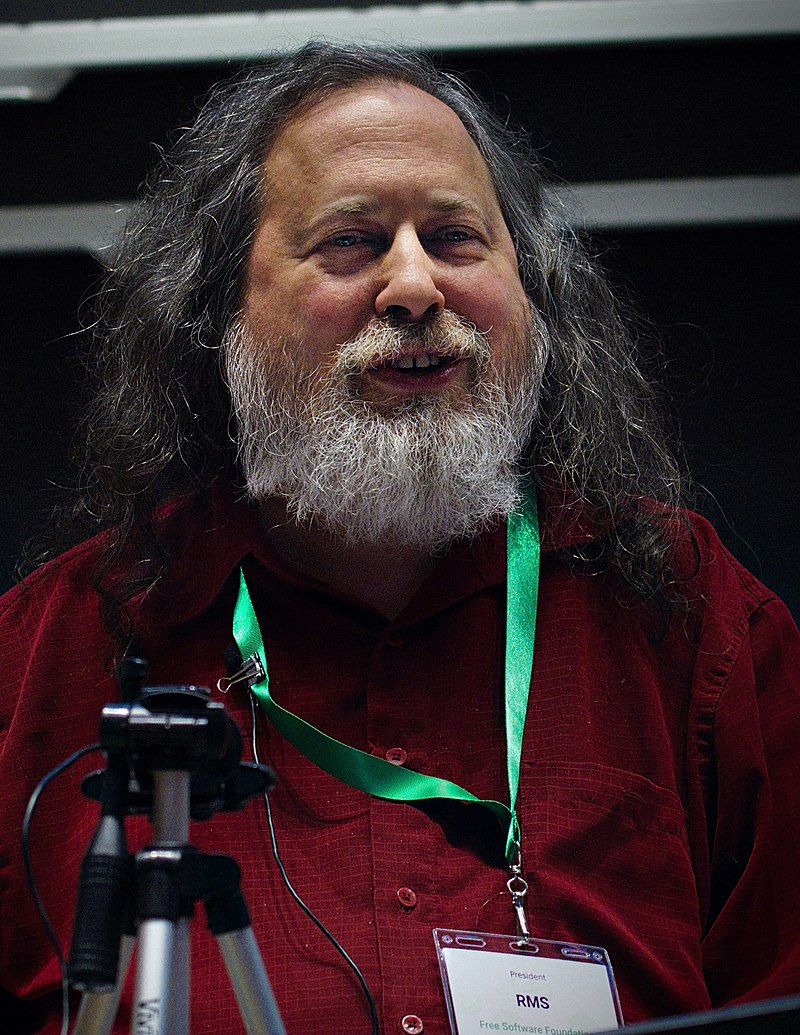
\includegraphics[width=0.25\textwidth]{images/rms.jpg}
		\end{center}
		\caption{Lovely Stallman}
	\end{figure}
\end{frame}

\begin{frame}{Why FOSS?}
	\begin{itemize}
		\item \textbf{Freedom and control:}  FOSS provides users with the freedom to run, modify, and \textit{hack} the software.
			Users have control over the software they use, allowing them to adapt it to their specific needs.
		\item \textbf{Transparency:} The source code of FOSS is open and accessible to anyone. This transparency allows
			users to inspect the code for security vulnerabilities, understand how the software works,
			and verify that it behaves as intended. This transparency can enhance trust and security.
		\item \textbf{Community Collaboration:} FOSS projects often involve collaboration among a global community of developers.
			This collaborative model can lead to more robust, secure, and innovative software. Users can contribute 
			to the improvement of the software or customize it to suit their requirements.
	\end{itemize}
\end{frame}

\begin{frame}{Why FOSS?}
	\begin{itemize}
		\item \textbf{Fighting monopoly:} FOSS promotes the decentralization of control by enabling a diverse and 
			global community of contributors. When a software project is open source, it's not tied 
			to the decisions and control of a single company or entity. This helps prevent a monopoly 
			on development and decision-making. 
	\end{itemize}
\end{frame}

\begin{frame}{Notable pieces of software:}
	In the following slides, some notable Free and open source projects will be presented:
\end{frame}

\begin{frame}{LibreOffice}
	A free and powerful office suite. Has a user-friendly interface and is cross-platform.
	\begin{figure}[]
		\begin{center}
			
\includegraphics[width=0.45\textwidth]{images/LibreOffice.png}
		\end{center}
		\caption{The LibreOffice Logo}
	\end{figure}
\end{frame}

\begin{frame}{GIMP}
	A cross-platform image editor available for GNU/Linux, macOS, Windows and more operating 
	systems. It is free software, you can change its source code and distribute your changes. 
	\begin{figure}
		\begin{center}
			
\includegraphics[width=0.45\textwidth]{images/gimp.png}
		\end{center}
		\caption{The lovely GIMP logo}
	\end{figure}
\end{frame}

\begin{frame}{What is UNIX?}
	Unix is a powerful, multiuser, multitasking operating system originally developed in 
	the 1960s and 1970s at Bell Labs (the research and development subsidiary of AT\&T).
	It has since become a widely used operating system, forming the basis for many other 
	operating systems, including Linux and macOS.
	\begin{figure}
		\begin{center}
			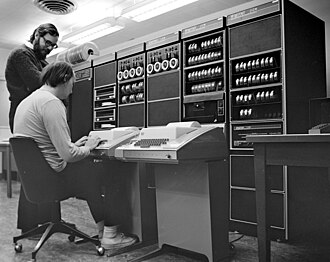
\includegraphics[width=0.45\textwidth]{images/unix.png}
		\end{center}
		\caption{Ken Thompson and Dennis Ritchie}
	\end{figure}
\end{frame}

\begin{frame}{What is GNU?}
	A Unix-like operating system. That means it is a collection of many programs: applications, libraries,
	developer tools, even games.

	The name “GNU” is a recursive acronym for “GNU's Not Unix.”. GNU is Unix-like not directly 
	a descendant of Unix itself.
	\begin{figure}
		\begin{center}
			
\includegraphics[width=0.25\textwidth]{images/gnu.png}
		\end{center}
		\caption{The GNU logo}
	\end{figure}
\end{frame}

\begin{frame}{The Unix timeline}
	\begin{figure}
		\begin{center}
			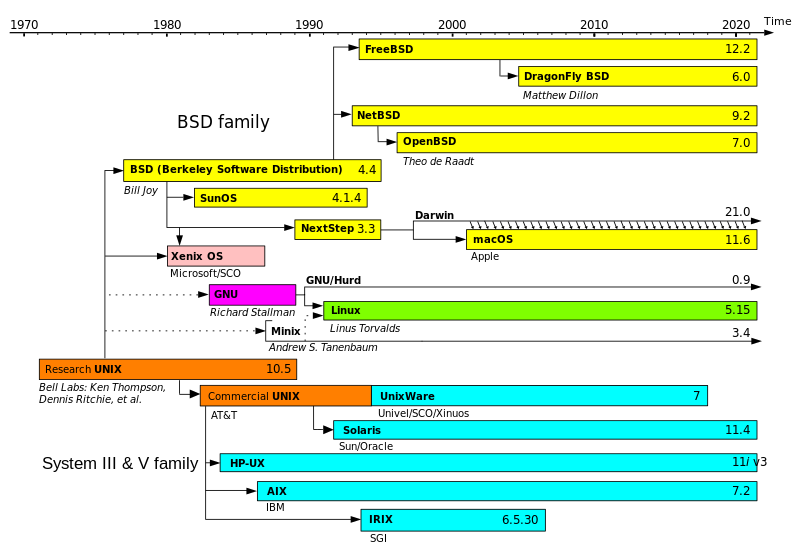
\includegraphics[width=0.95\textwidth]{images/Unix_timeline.png}
		\end{center}
	\end{figure}
\end{frame}

\begin{frame}{What is Linux?}
	Linux is an open-source, Unix-like operating system kernel first created by Linus Torvalds 
	in 1991. The kernel is the core component of an operating system that interacts with the 
	hardware and manages system resources.
	\begin{figure}
		\begin{minipage}{0.45\textwidth}
			\centering
			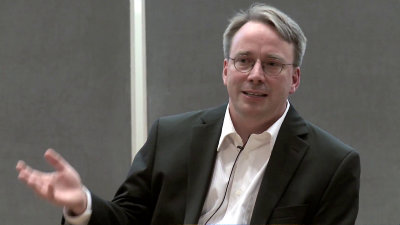
\includegraphics[width=0.9\textwidth]{images/torvalds.jpg}
			\caption{Torvalds hating Nvidia}
		\end{minipage}\hfill
		\begin{minipage}{0.45\textwidth}
			\centering
			
\includegraphics[width=0.7\textwidth]{images/tux.png}
			\caption{Lovely Tux}
		\end{minipage}
	\end{figure}
\end{frame}

\begin{frame}{Controversial notation}
		Referring to GNU/Linux operating system simply as "Linux" is a common but controversial
		practice. The controversy stems from the fact that the operating system is a combination 
		of the Linux kernel, developed by Linus Torvalds, and the GNU operating system, developed 
		by the Free Software Foundation (FSF) led by Richard Stallman.
\end{frame}

\begin{frame}{Distributions}
		A Linux distribution constitutes a comprehensive operating system encompassing the Linux kernel,
		system libraries, utilities, application software, and a package management system. It is crafted
		by diverse software components from various origins and bundling them to deliver an
		integrated and user-friendly computing environment.
		Here are some notable distributions:
\end{frame}

\begin{frame}{Debian}
		Also known as Debian GNU/Linux, is a Linux distribution composed of free and open-source 
		software, developed by the community-supported Debian Project, which was established by 
		Ian Murdock on August 16, 1993.
		\begin{figure}
			\begin{center}
				
\includegraphics[width=0.45\textwidth]{images/debian-logo.jpg}
			\end{center}
			\caption{Debian logo}
		\end{figure}
		
\end{frame}

\begin{frame}{Fedora}
		A Linux distribution developed by the Fedora Project. It was originally
		developed in 2003 as a continuation of the Red Hat Linux project
		\begin{figure}
			\begin{center}
				
\includegraphics[width=0.25\textwidth]{images/fedora-logo.png}
			\end{center}
			\caption{Fedora logo}
		\end{figure}
\end{frame}

\begin{frame}{Arch}
		 An independently developed, x86-64 general purpose GNU/Linux distribution 
		 versatile enough to suit any role. Development focuses on simplicity, minimalism,
		 and code elegance.
		\begin{figure}
			\begin{center}
				
\includegraphics[width=0.65\textwidth]{images/arch-logo.png}
			\end{center}
			\caption{Arch Linux logo}
		\end{figure}
\end{frame}

\begin{frame}{Some facts about Arch}
		In vanilla Arch Linux installation, you are greeted with a simple shell to install
		your operating system.
		\begin{figure}
			\begin{center}
				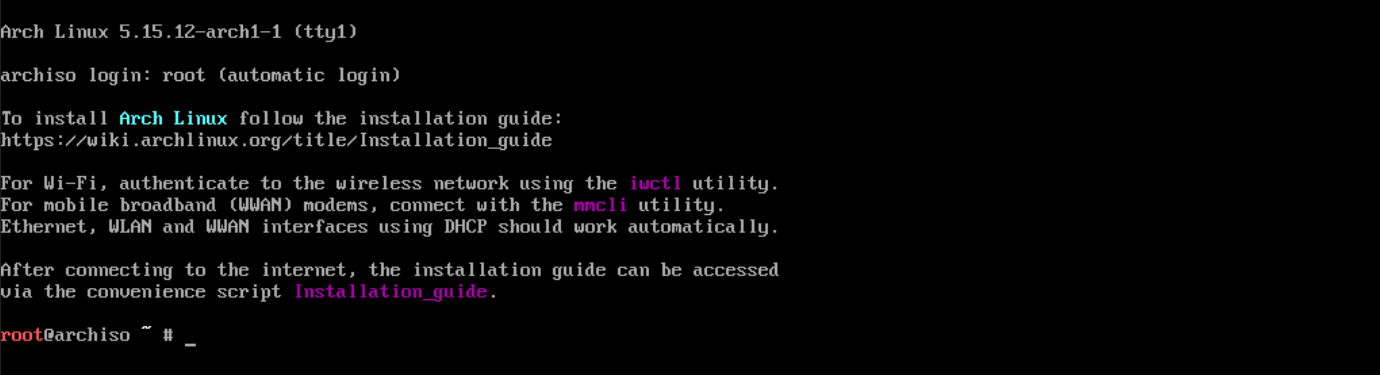
\includegraphics[width=0.95\textwidth]{images/arch-live.png}
			\end{center}
			\caption{Live USB shell}
		\end{figure}
\end{frame}

\begin{frame}{Extra Points}
		Provide a complete video of installing an Arch Linux setup. Explaining all the commands
		used in the process.

		Using the official Arch Wiki is recommended.
\end{frame}

\begin{frame}{Gentoo}
		a free operating system based on Linux that can be automatically optimized 
		and customized for just about any application or need. Extreme configurability,
		performance, and a top-notch user and developer community are all hallmarks of the Gentoo experience. 
		\begin{figure}
			\begin{center}
				
\includegraphics[width=0.25\textwidth]{images/gentoo-logo.png}
			\end{center}
			\caption{Gentoo logo}
		\end{figure}
\end{frame}

\begin{frame}{Rolling Release Distributions}
	In software development, rolling release is a model in which updates to a software are continuously rolled out, 
	rather than in batches of versions. This way the software always remains up to date. A rolling release distribution
	follows the same model, and it provides the latest Linux kernel and the software version as they are released.
\end{frame}

\begin{frame}{Packages}
	Software packages, or packages for short, is a collection of files and metadata that contains a specific software 
	application or program. It is designed to simplify the process of distributing, installing, and managing software 
	on a computer system.

	Packages may be stored in a remote server and be downloaded by users using \textit{package managers}
\end{frame}

\begin{frame}{Getting started}
    We will be covering the installation of the Parch Linux distribution. A distribution based on Arch that
    is good for a beginner as it doesn't require installing via the vanilla shell.

    It is recommended that as a beginner you install it first on a Virtual Machine such as VirtualBox
    and only after you are comfortable with it, you install it on your machine.
\end{frame}

\begin{frame}{Installation Process}
	The installation process should be pretty much straight-forward since everything is done using the
	GUI. Even the installer uses a GUI tool to automate the installation process.
\end{frame}

\begin{frame}{Users}
	\begin{itemize}
		\item In Linux, users and groups are fundamental components of the system's security and access control.

		\item User accounts are associated with specific privileges and settings.

		\item Each user has a home directory for personal files and configurations.
		\end{itemize}
\end{frame}

\begin{frame}{Groups}
	\begin{itemize}
		\item Groups are collections of users with similar permissions or roles.

		\item Group accounts help manage access to files, directories, and resources.
		\item You can see the groups that your user is in using the \texttt{groups}
	command.
\end{itemize}
\end{frame}

\begin{frame}{Get to know groups}
	Arch Wiki provides a list of predefined groups and their permissions
	in the \textit{Users and groups} section.
\end{frame}

\begin{frame}{Superuser (Root)}
	    In Linux, the superuser, commonly referred to as "root," is the administrative account with elevated privileges.
\end{frame}

\begin{frame}{Role of the Superuser}
	Some roles of the Superuser include:
	\begin{enumerate}
		\item \textbf{Administrative Privileges:}     The root user has the highest level of access and can perform any administrative task on the system.
		\item \textbf{System Configuration:}     Responsible for configuring system-wide settings and making critical changes.
		\item \textbf{Filesystem Access:}     Can access and modify any file or directory on the system.
	\end{enumerate}
\end{frame}

\begin{frame}{Accessing the root user}
	\begin{enumerate}
		\item \textbf{Using 'su' Command:} Users can switch to the root account using the 'su' (substitute user) command.
		\item \textbf{Using 'sudo' Command:} for granting temporary administrative privileges.
			
			\texttt {sudo command}
	\end{enumerate}
\end{frame}

\begin{frame}{FHS}
	The Filesystem Hierarchy Standard (FHS) is a set of conventions for the layout of directories in Unix-like operating systems. It provides a standardized structure, organization, and naming conventions for files and directories, promoting consistency and interoperability across different Unix and Unix-like systems.
\end{frame}

\begin{frame}{An overview of FHS}
	\begin{enumerate}
		\item \textbf{Root Directory (/):} 
			\begin{itemize}
				\item The top-level directory in the filesystem hierarchy.
				\item All other directories and files are organized beneath the root directory.
			\end{itemize}
	\item {\textbf{/bin (Binaries):}}
			\begin{itemize}
				\item Essential user command binaries (executable files) required for system boot and repair.
			\end{itemize}
		\item {\textbf{/boot:}}
			\begin{itemize}
				\item Files needed for the boot process, including the kernel, bootloader configuration, and other boot-related files.
			\end{itemize}
		\item \textbf{/dev (Device Files):}
			\begin{itemize}
				\item Device files representing hardware devices and pseudo-devices.
				\item Provides a interface for user-space programs to interact with the kernel and devices.
			\end{itemize}
	\end{enumerate}
\end{frame}

\begin{frame}{An overview of FHS}
	\begin{enumerate}
		\setcounter{enumi}{4}
		\item \textbf{/etc (Configuration Files):} 
			\begin{itemize}
				\item System-wide configuration files and shell scripts.
				\item Contains configuration files for the system and installed applications.
			\end{itemize}
		\item \textbf{/home:} 
			\begin{itemize}
				\item Home directories for regular users.
				\item Each user has a dedicated subdirectory under /home.
			\end{itemize}
		\item \textbf{/root:}
			\begin{itemize}
				\item     Home directory for the root user (superuser/administrator).
			\end{itemize}
		\end{enumerate}
		You can read more about the FHS in Arch Linux by visiting the file-hierarchy(7) Arch manual page
\end{frame}

\begin{frame}{Package manager}
	\begin{itemize}
		\item Arch Linux's package management enables users to have access to new
	software with ease.
		\item It uses a package manager called \textbf{pacman} that
			handles everything related to package installations.
		\item This system allows users to install software within
			one command!
	\end{itemize}
\end{frame}

\begin{frame}{Installing packages}
	Installing a package is as simple as using the \texttt{pacman -Syy} command followed by the package name:
	
	You can find the name of the packages simply by searching the name
	of the package followed by Arch Linux in Google.
\end{frame}

\begin{frame}{Handling dependencies}
	    Pacman efficiently handles dependencies, automatically installing or removing them as needed. So dependency errors are very unlikely!
\end{frame}

\begin{frame}{Removing packages}
	Removing packages is straightforward with \texttt{pacman -Rns} followed by the package name.
\end{frame}

\begin{frame}{System upgrades}
It's quite important to keep your install updated by running \texttt{sudo pacman -Syu} once in a while to make sure you have the latest updates!
\end{frame}

\begin{frame}{Installing a new shell}
	Let's go through installing a new shell called "fish" in our newly installed OS. You will be learning how to use
	the Arch Wiki to go through the process.
\end{frame}

\begin{frame}{The AUR}
    The Arch User Repository (AUR) is a community-driven repository for Arch Linux, providing a vast collection of user-contributed packages beyond those in the official repositories. This decentralized and collaborative platform enhances the flexibility and diversity of software available to Arch Linux users
\end{frame}

\begin{frame}{Key Features of the AUR}
\begin{itemize}
	\item AUR allows Arch Linux users to share and distribute packages they've created or modified.

	\item     The AUR is maintained by the Arch Linux community, reflecting the collaborative and open-source nature of the Arch Linux ecosystem.

	\item     Offers a wide array of packages, including bleeding-edge software, beta releases, and software not available in the official repositories.
\end{itemize}
\end{frame}

\begin{frame}{Using the AUR}
	There are typically two ways to use the packages from the AUR

	\begin{enumerate}
		\item Use a helper tool like yay (Installation described in class)
		\item Manually installing AUR packages
	\end{enumerate}
\end{frame}

\begin{frame}{Getting more shell-friendly}
	Proficiency in the command line is a must for a Linux user. It gives the user the power to do \textit{anything} they want with their computer.
	We will be going through some basic commands usually available in most of the distributions.
\end{frame}

\begin{frame}[fragile]{cd (Change Directory)}
	Very basic command to change the current working directory.
\begin{lstlisting}
cd someDirectory
cd ../
cd ../SomePreviousFolder
\end{lstlisting}
\end{frame}

\begin{frame}[fragile]{cp (copy files and directories)}
	\textbf{Command used to copy files and directories.}
\begin{lstlisting}
cp file1.c copyOfFile1.c
cp file1.c someDirectory/copyOfFile1
cp -r someDirectory copyOfSomeDirectory
\end{lstlisting}
\par{Make sure to take a look at the available arguments via \lstinline{man cp}}
\end{frame}

\begin{frame}[fragile]{rm (Remove Files and Directories)}
  \textbf{Delete files and directories with caution!}

    \begin{lstlisting}[frame=none]
  rm file1.txt          # Removes file1.txt
  rm *.txt              # Removes all .txt files in current directory
  rm -r someDirectory  # Removes directory "someDirectory" and its contents (recursive)
  rm -f file2.txt      # Forces deletion without confirmation (caution!)
  \end{lstlisting}

  \textbf{Remember:} Deleted files are usually gone forever. Use `man rm` for detailed options and flags.

  \begin{itemize}
    \item \textbf{Backup important data before using `rm`!}
    \item Double-check filenames before running the command.
  \end{itemize}
\end{frame}

\begin{frame}[fragile]{mv (Move files and directories)}
  \textbf{Safely move files and directories with `mv`!}

    \begin{lstlisting}
  mv file1.txt newFile.txt # Renames file1.txt to newFile.txt
  mv file2.txt someDirectory # Moves file2.txt to directory "someDirectory"
  mv -r oldDirectory newDirectory # Moves directory "oldDirectory" to "newDirectory" (including contents)
  mv *.* .. # Moves all files in current directory to parent directory
  \end{lstlisting}

  \textbf{Remember:} Files and directories are relocated, not copied.

  \begin{itemize}
    \item Use `mv` instead of `cp` when you want to change the location, not duplicate files.
  \end{itemize}

  \textbf{Bonus tip:} Use `man mv` for detailed options like overwriting existing files.

\end{frame}

\begin{frame}[fragile]{mkdir (Master of Directory Creation)}

  \textbf{Craft your file system with `mkdir`!}

  \begin{lstlisting}[frame=none]
  mkdir directory_name # Creates a new directory named "directory_name"
  mkdir -p /path/to/nested/directory # Creates all necessary directories in the path, even nested ones
  mkdir -v /data/backup # Displays a verbose message confirming directory creation
  \end{lstlisting}

  \textbf{The architect of your file system organization! `mkdir` shapes your storage landscape by building new directories wherever you need them.}

  \begin{itemize}
    \item Organize your files into structured and accessible directories.
    \item Streamline workflow by grouping related files in dedicated folders.
    \item Craft custom directory structures for specific projects or applications.
    \item Stay informed with verbose messages or confirmation prompts for precise control.
  \end{itemize}

  \textbf{Remember:`mkdir` creates directories, but it doesn't automatically populate them with files.}

\end{frame}


\begin{frame}[fragile]{ls (List Directory Contents)}
  \textbf{Peek into your directories with `ls`!}

  \begin{lstlisting}[frame=none]
  ls                           # Lists all files and directories in current directory
  ls -l                        # Lists files and directories with detailed information (long format)
  ls -a                        # Lists all files, including hidden ones (dot files)
  ls -R                        # Lists files and directories recursively (subdirectories included)
  ls file1.txt file2.jpg       # Lists specific files (space-separated)
  ls someDirectory/            # Lists contents of a specific directory
  \end{lstlisting}

  \textbf{Remember:} `ls` only shows what's there, it doesn't modify anything.

  \textbf{Bonus tip:} Combine options for customized listings! (e.g., `ls -laR`)

\end{frame}

\begin{frame}[fragile]{pwd (Print Working Directory)}
  \textbf{Know where you are with `pwd`!}

  \begin{lstlisting}[frame=none]
  pwd                    # Prints the full path of the current working directory
  \end{lstlisting}

  \textbf{Simple but essential! `pwd` quickly tells you your current location within the file system hierarchy.}

  \begin{itemize}
    \item Use `pwd` to regain your bearings when navigating directories.
    \item Combine `pwd` with other commands like `cd` for efficient navigation.
    \item Knowing your `pwd` is crucial for referencing files and directories.
  \end{itemize}

  \textbf{Remember:} `pwd` only displays the path, it doesn't change your location.

\end{frame}

\begin{frame}[fragile]{echo (Speak Up!)}
  \textbf{Make your voice heard with `echo`!}

  \begin{lstlisting}[frame=none]
  echo "This is a simple message." # Prints the message directly to the console.
  echo $USER # Prints your username.
  echo $PWD # Prints your current working directory.
  echo -n "No newline here" # Suppresses the newline character after the message.
  echo -e "Line 1\nLine 2" # Enables escape sequences like line breaks.
  \end{lstlisting}

  \textbf{Versatile and powerful! `echo` displays text, variables, and even manipulates output.}

  \begin{itemize}
    \item Use `echo` to display messages for user information or debugging.
    \item Combine `echo` with variables to personalize your output.
    \item Leverage escape sequences to format your text with line breaks, tabs, and more.
  \end{itemize}

  \textbf{Remember:} `echo` only prints, it doesn't affect file content or modify the system.
\end{frame}

\begin{frame}[fragile]{ping (Check Your Network Pulse)}
	\textbf{Test your network connection with a ping!}

  \begin{lstlisting}[frame=none]
  ping google.com # Checks connectivity to Google
  ping 8.8.8.8 # Pings Google's DNS server directly using its IP address
  ping -t example.com # Continuously pings until stopped with Ctrl+C
  \end{lstlisting}

  \textbf{Essential for network troubleshooting! `ping` measures the round-trip time of packets to assess connectivity and identify network issues.}

  \begin{itemize}
    \item Use `ping` to diagnose connection problems like slow network speeds or outages.
  \end{itemize}
\end{frame}

\begin{frame}[fragile]{curl (Get Data From the Web)}
  \textbf{Reach out to the internet with `curl`!}

  \begin{lstlisting}[frame=none]
  curl https://www.example.com # Retrieves website content from URL
  curl -O https://example.com/image.png # Saves downloaded file as "image.png"
  \end{lstlisting}

  \textbf{Powerful and versatile! `curl` interacts with web servers to retrieve data, download files, and even send information.}

  \begin{itemize}
    \item Use `curl` to fetch website content for analysis or scraping.
    \item Download files directly from the internet with custom filenames.
    \item Access APIs to retrieve or send data in various formats.
  \end{itemize}

\end{frame}

\begin{frame}[fragile]{tar (Tape Archive)}
  \textbf{Pack up and unpack your files with `tar`!}

  \begin{lstlisting}[frame=none]
  tar -cf archive.tar file1.txt file2.jpg # Creates archive "archive.tar" with two files
  tar -xvf archive.tar # Extracts files from archive "archive.tar" to current directory
  tar -czf backup.tar.gz someDirectory # Creates compressed archive with directory contents
  tar -xzvf compressed_files.tar.gz -C anotherDirectory # Extracts files to specific directory
  tar -tf some_archive.tar # Lists files within the archive without extracting them
  \end{lstlisting}

  \textbf{Versatile and efficient! `tar` bundles files and directories into compressed archives for easy storage, transfer, and backup.}

  \begin{itemize}
    \item Pack up directories with their complete structure for easy restoration later.
    \item Combine `tar` with compression algorithms like gzip or bzip2 for smaller archives.
  \end{itemize}
\end{frame}

\begin{frame}[fragile]{lsblk (List Your Block Devices)}
  \textbf{Map Your Storage Landscape with `lsblk`!}

  \begin{lstlisting}[frame=none]
  lsblk # Lists all available block devices
  lsblk /dev/sda # Focuses on a specific device
  lsblk -f # Lists all partitions and subdevices
  lsblk -p # Displays detailed partition information
  \end{lstlisting}

  \textbf{`lsblk` provides a comprehensive overview of your block devices, including disks, partitions, and optical drives.}

  \begin{itemize}
    \item Identify connected drives, their types, and file systems.
    \item Check available sizes and usage for informed storage management.
  \end{itemize}
\end{frame}


\begin{frame}[fragile]{mount \& umount (Mount Your File Systems)}
  \textbf{Connect and Access Your Storage with `mount`!}

  \begin{lstlisting}[frame=none]
  mount /dev/sda1 /home # Mounts partition /dev/sda1 to /home directory
  umount /mnt/usb # Unmounts the USB drive
  \end{lstlisting}

  \textbf{The gateway to your data! `mount` attaches external devices, network shares, and even remote storage to your system, making them readily accessible like local files.}

  \begin{itemize}
    \item Connect your external hard drives, USB sticks, and network shares for seamless access.
    \item Control mount options like read/write access or execution permissions for added security.
    \item Easily manage and detach mounted storage devices with the `umount` command.
  \end{itemize}
\end{frame}

\begin{frame}[fragile]{du (Disk Usage Detective)}
  \textbf{Uncover storage hogs with `du`!}

  \begin{lstlisting}[frame=none]
  du -sh current_directory # Shows disk usage summary for current directory and subdirectories
  du -sh /home/* # Analyzes disk usage for all directories in /home
  du -sb file1.txt file2.jpg # Displays size in bytes for specific files
  du -h /media/usb # Estimates usage in human-readable format (e.g., MB, GB)
  \end{lstlisting}

  \textbf{`du` digs into your storage, revealing the culprits consuming valuable disk space.}

  \begin{itemize}
    \item Track down storage-hungry files and directories for efficient management.
    \item Analyze disk usage across different locations and identify potential cleanup targets.
    \item Get precise size information for specific files and directories.
  \end{itemize}
\end{frame}

\begin{frame}[fragile]{df (Disk Freeway Inspector)}
  \textbf{Monitor your storage health with `df`!}

  \begin{lstlisting}[frame=none]
  df # Shows free and used space for all mounted file systems
  df -h /home # Displays disk usage in human-readable format for specific mount point
  df -T # Displays file system type for each mounted device
  \end{lstlisting}

  \textbf{`df` keeps you informed about the available and occupied space on your file systems, ensuring smooth operation and preventing disk space exhaustion.}

  \begin{itemize}
    \item Stay ahead of disk space limitations with real-time usage information.
    \item Identify specific file systems nearing capacity for proactive management.
    \item Analyze physical disk utilization for deeper understanding of storage allocation.
    \item Verify file system types for compatibility and troubleshooting purposes.
  \end{itemize}
\end{frame}

\begin{frame}[fragile]{whoami (Identify Yourself)}

  \textbf{Unmask your identity with `whoami`!}

  \begin{lstlisting}[frame=none]
  whoami # Reveals your current username
  \end{lstlisting}

  \textbf{Know who you are! `whoami` sheds light on your system identity, essential for managing permissions, tracking logs, and understanding your context within the system.}

  \begin{itemize}
    \item Quickly confirm your current username in any terminal session.
  \end{itemize}
\end{frame}

\begin{frame}[fragile]{fd (Find It! The File Detective)}

  \textbf{Track down files with effortless precision using `fd`!}

  \begin{lstlisting}[frame=none]
  fd "keyword" # Finds all files containing the keyword in their name or content
  fd --glob "*.txt" current_directory # Searches for all text files in the current directory
  \end{lstlisting}

  \textbf{`fd` becomes your trusty companion in navigating your file system, uncovering hidden files, and organizing your digital landscape.}

  \begin{itemize}
    \item Locate files by keyword, extension, or regular expression with unmatched efficiency.
    \item Explore specific directories or delve deep into files with recursive searching.
    \item Fine-tune your search with options like ignoring hidden files and case sensitivity.
  \end{itemize}
\end{frame}


\begin{frame}[fragile]{md5sum (Verify Integrity! The Checksum Sleuth)}

  \textbf{Ensure data integrity and detect file alterations with `md5sum`!}

  \begin{lstlisting}[frame=none]
  md5sum filename # Computes and displays the MD5 checksum of the file
  md5sum -c checksum_file # Verifies the integrity of files based on a checksum file
  \end{lstlisting}

  \textbf{`md5sum` is your forensic tool for confirming that file contents have not been tampered with.}

  \begin{itemize}
    \item Generate MD5 hashes to establish a baseline for file contents.
    \item Verify download integrity to prevent malicious tampering.
    \item Automate integrity checks in scripts for batch verification.
  \end{itemize}
\end{frame}

\begin{frame}[fragile]{grep (Global Regular Expression Print)}

  \textbf{Unleash the power of text pattern matching with `grep`!}

  \begin{lstlisting}[frame=none]
  grep "pattern" filename # Search for a specific pattern in a file
  grep -r "pattern" /path/to/directory # Recursive search in a directory
  grep -i "case-insensitive" file.txt # Perform case-insensitive matching
  grep -n "pattern" file.txt # Display line numbers along with matching lines
  grep -E "regex pattern" file.txt # Use extended regular expressions for complex patterns
  \end{lstlisting}
  
\end{frame}

\begin{frame}{More about grep!}
  \textbf{Effortlessly sift through text files, pinpointing crucial information with `grep`!}

  \begin{itemize}
    \item Find lines containing specific patterns in files.
    \item Explore directories recursively for pattern-matching across multiple files.
    \item Ignore case for flexible and inclusive pattern matching.
    \item Quickly locate line numbers along with matching content.
    \item Harness the power of extended regular expressions for intricate pattern matching.
  \end{itemize}

  \textbf{Pro Tip: Combine `grep` with other commands for advanced text processing! More on this soon!}

\end{frame}

\begin{frame}[fragile]{wc (Word Count)}

  \textbf{Get a comprehensive analysis of your text files with `wc`!}

  \begin{lstlisting}[frame=none]
  wc filename # Display the count of lines, words, and characters in a file
  wc -l filename # Count the number of lines in a file
  wc -w filename # Count the number of words in a file
  wc -c filename # Count the number of characters in a file
  \end{lstlisting}

\end{frame}

\begin{frame}{More about wc!}

  \textbf{Efficiently analyze the structure and content of your text files using `wc`!}

  \begin{itemize}
    \item Obtain a summary of lines, words, and characters in a file.
    \item Focus on specific metrics such as line count, word count, or character count.
    \item Customize your analysis for a detailed understanding of your text data.
    \item Ideal for assessing the size and complexity of documents or code files.
    \item Integrate `wc` into scripts or pipelines for automated data analysis.
  \end{itemize}

  \textbf{Pro Tip: Combine `wc` with other commands to build powerful text processing workflows!}

\end{frame}

\begin{frame}[fragile]{Piping in Bash}

  \textbf{Streamlining Workflows with Piping}

  \begin{itemize}
    \item Leverage the power of pipes to connect the output of one command to the input of another.
    \item Enhance efficiency by creating seamless data flows between commands.
    \item Use the pipe operator \text{\textbar} to chain commands together in a single line.
  \end{itemize}

  \begin{lstlisting}[frame=none]
  command1 | command2
  \end{lstlisting}

  \textbf{Example:}

  \begin{lstlisting}[frame=none]
  ls -l | grep "file" | wc -l
  \end{lstlisting}

\end{frame}

\begin{frame}{\textbf{Benefits of Piping:}}
  \begin{itemize}
    \item \textbf{Modularity:} Combine simple commands for complex operations.
    \item \textbf{Efficiency:} Avoid creating intermediate files by passing data directly.
    \item \textbf{Flexibility:} Easily customize and extend functionality with various command combinations.
  \end{itemize}

  \textbf{Master the art of piping for a more fluid and powerful command-line experience in Bash!}

\end{frame}

\begin{frame}[fragile]{More Examples of Piping}

  \textbf{Example 1: Count lines with a specific word in a log file:}
  \begin{lstlisting}[frame=none]
  cat logfile.txt | grep "error" | wc -l
  \end{lstlisting}

  \textbf{Example 2: List top 10 largest files in a directory:}
  \begin{lstlisting}[frame=none]
  du -h | sort -rh | head -n 10
  \end{lstlisting}

  \textbf{Example 3: Find `.txt` files modified in the last 7 days and count:}
  \begin{lstlisting}[frame=none]
  find . -name "*.txt" -mtime -7 | wc -l
  \end{lstlisting}

\end{frame}

\begin{frame}{UNIX Philosophy and modularity}
    In the previous slides, a philosophy called the \textit{UNIX Philosophy} really shines. Below are two that you might really relate to:
    \begin{itemize}
        \item Make each program do one thing well. To do a new job, build afresh rather than complicate old programs by adding new "features".
        \item Expect the output of every program to become the input to another, as yet unknown, program. Don't clutter output with extraneous information. Avoid stringently columnar or binary input formats. Don't insist on interactive input.
    \end{itemize}
\end{frame}

\begin{frame}[fragile]{Understanding stdin in Bash}

  \textbf{Standard Input (stdin)}

  \begin{itemize}
    \item Represents the input stream where data is read by a command.
    \item Numbered as `0`.
  \end{itemize}

  \textbf{Usage in Commands:}

  \begin{itemize}
    \item Input often received from the keyboard or redirected from a file.
  \end{itemize}
\end{frame}

\begin{frame}[fragile]{Understanding stdout in Bash}

  \textbf{Standard Output (stdout)}

  \begin{itemize}
    \item Represents the output stream where a command displays its results.
    \item Numbered as `1`.
  \end{itemize}

  \textbf{Usage in Commands:}

  \begin{itemize}
    \item Output is typically displayed in the terminal or redirected to a file.
  \end{itemize}

  \begin{lstlisting}[frame=none]
  # Output to stdout
  echo "Hello, World!"
  \end{lstlisting}

\end{frame}

\begin{frame}[fragile]{Role of Stdout and Stdin in Piping}

  \textbf{Piping in Bash}

  \begin{itemize}
      \item \textbf{Piping (`\text{\textbar}`):} Connects the stdout of one command to the stdin of another.
    \item Enables the seamless flow of data between commands.
  \end{itemize}

  \textbf{Example Piping:}

  \begin{lstlisting}[frame=none]
  command1 | command2
  \end{lstlisting}

  \textbf{How it Works:}

  \begin{enumerate}
    \item Output from \textbf{command1} is sent to stdout.
    \item Piping (`\text{\textbar}`) takes that stdout and directs it as input to \textbf{command2} via stdin.
    \item \textbf{command2} processes the input received from \textbf{command1}.
  \end{enumerate}
\end{frame}

\begin{frame}[fragile]{Standard Output Redirection (`$>$`)}

  \textbf{Redirects the stdout (standard output) of a command to a file.}

  \begin{lstlisting}[frame=none]
  command > output.txt
  \end{lstlisting}

  \textbf{Example:}

  \begin{lstlisting}[frame=none]
  echo "Hello, World!" > greeting.txt
  \end{lstlisting}

\end{frame}

\begin{frame}[fragile]{Standard Input Redirection (`$<$')}

  \textbf{Redirects the stdin (standard input) of a command from a file.}

  \begin{lstlisting}[frame=none]
  command < input.txt
  \end{lstlisting}

  \textbf{Example:}

  \begin{lstlisting}[frame=none]
  cat < data.txt
  \end{lstlisting}

\end{frame}

\begin{frame}[fragile]{Combining Redirections}

  \textbf{Redirect both stdout and stderr to a file.}

  \begin{lstlisting}[frame=none]
  command < output_and_error.txt > anotherFile.txt
  \end{lstlisting}

  \textbf{Understanding redirection is essential for effective command-line operations in Bash!}

\end{frame}
%
% \begin{frame}{Introduction to Bash Scripting}
%
%   \textbf{What is Bash?}
%
%   \begin{itemize}
%     \item \textbf{Bash:} Bourne Again SHell is a Unix shell and command language.
%     \item Default shell for most Linux distributions and macOS.
%     \item Provides a command-line interface (CLI) for interacting with the operating system.
%   \end{itemize}
%
% \end{frame}
%
% \begin{frame}{Why Bash Scripting?}
%
%   \begin{itemize}
%     \item \textbf{Automation:} Streamline repetitive tasks by scripting them.
%     \item \textbf{Customization:} Tailor your command-line environment.
%     \item \textbf{Programming:} Learn scripting for system administration and beyond.
%   \end{itemize}
%
% \end{frame}

\begin{frame}{File Ownership in Linux}

  \textbf{Every File in Linux Has Two Owners:}

  \begin{itemize}
    \item \textbf{User Owner (User):} The individual who owns the file and has specific access rights.
    \item \textbf{Group Owner (Group):} The group to which the file belongs, and users in this group may have shared access rights.
  \end{itemize}

\end{frame}

\begin{frame}[fragile]{Commands to View Ownership}

  \textbf{Commands to View Ownership:}

  \begin{itemize}
    \item \textbf{`ls -l` (Long Format):} Displays detailed information including user and group ownership.
    \item \textbf{Example:} \\
      \begin{lstlisting}[frame=none]
      -rw-r--r-- 1 john users  4096 Dec 11 17:22 example.txt
      \end{lstlisting}
      \textbf{Owner (`john`), Group (`users`)}
  \end{itemize}

\end{frame}

\begin{frame}[fragile]{Changing Ownership}

  \textbf{Changing Ownership:}

  \begin{itemize}
    \item \textbf{`chown`:} Changes the user and/or group ownership of files.
    \item \textbf{Example:} \\
      \begin{lstlisting}[frame=none]
      chown newuser:newgroup file.txt
      \end{lstlisting}
  \end{itemize}

\end{frame}



\begin{frame}{Permission Bits in Unix-like Systems}

  \textbf{Introduction to Permission Bits:}

  \begin{itemize}
    \item In Unix-like systems, files and directories have associated permission bits that control access.
    \item Permissions are assigned to three categories: Owner, Group, and Others.
    \item Each category has three permission bits: Read (`r`), Write (`w`), and Execute (`x`).
  \end{itemize}

\end{frame}

\begin{frame}{Permission Representation}

  \textbf{Permission Representation:}

  \begin{itemize}
    \item Permissions are often represented as a sequence of three characters for each category.
    \item Example: `rw-` indicates read and write permissions, but no execute permission.
  \end{itemize}

\end{frame}

\begin{frame}{Permission Notation}

  \textbf{Permission Notation:}

  \begin{itemize}
    \item Numeric notation (Octal): Each permission bit is assigned a numeric value (4 for read, 2 for write, 1 for execute), and the sum represents the permission set.
    \item Example: `rw-` becomes `6` in octal notation (4 for read + 2 for write).
  \end{itemize}

\end{frame}

\begin{frame}{Setting and Changing Permissions}

  \textbf{Setting and Changing Permissions:}

  \begin{itemize}
    \item Permissions can be set using commands like `chmod`.
    \item Example: `chmod 755 filename` gives read, write, and execute permissions to the owner, and read and execute permissions to the group and others.
  \end{itemize}

\end{frame}









\end{document}
